\chapter{Analyse performance}
\label{chapter-4}

%Résultats du calcul de la puissance reçue et du débit binaire dans l'appart

%Suggestions placement


\section{Résultats}

Les résultats ont été réalisés avec la simulation à sa plus haute résolution (soit des cellules de $0,0625\mathrm{m}\times0,0625\mathrm{m}$).

% ---- salon ----
\subsection{Emplacement par défaut (salon)}
La station de base se trouve en (9.4, 7)m.

\subsubsection{Sans ascenseur}

\begin{figure}[H]
    \centering
    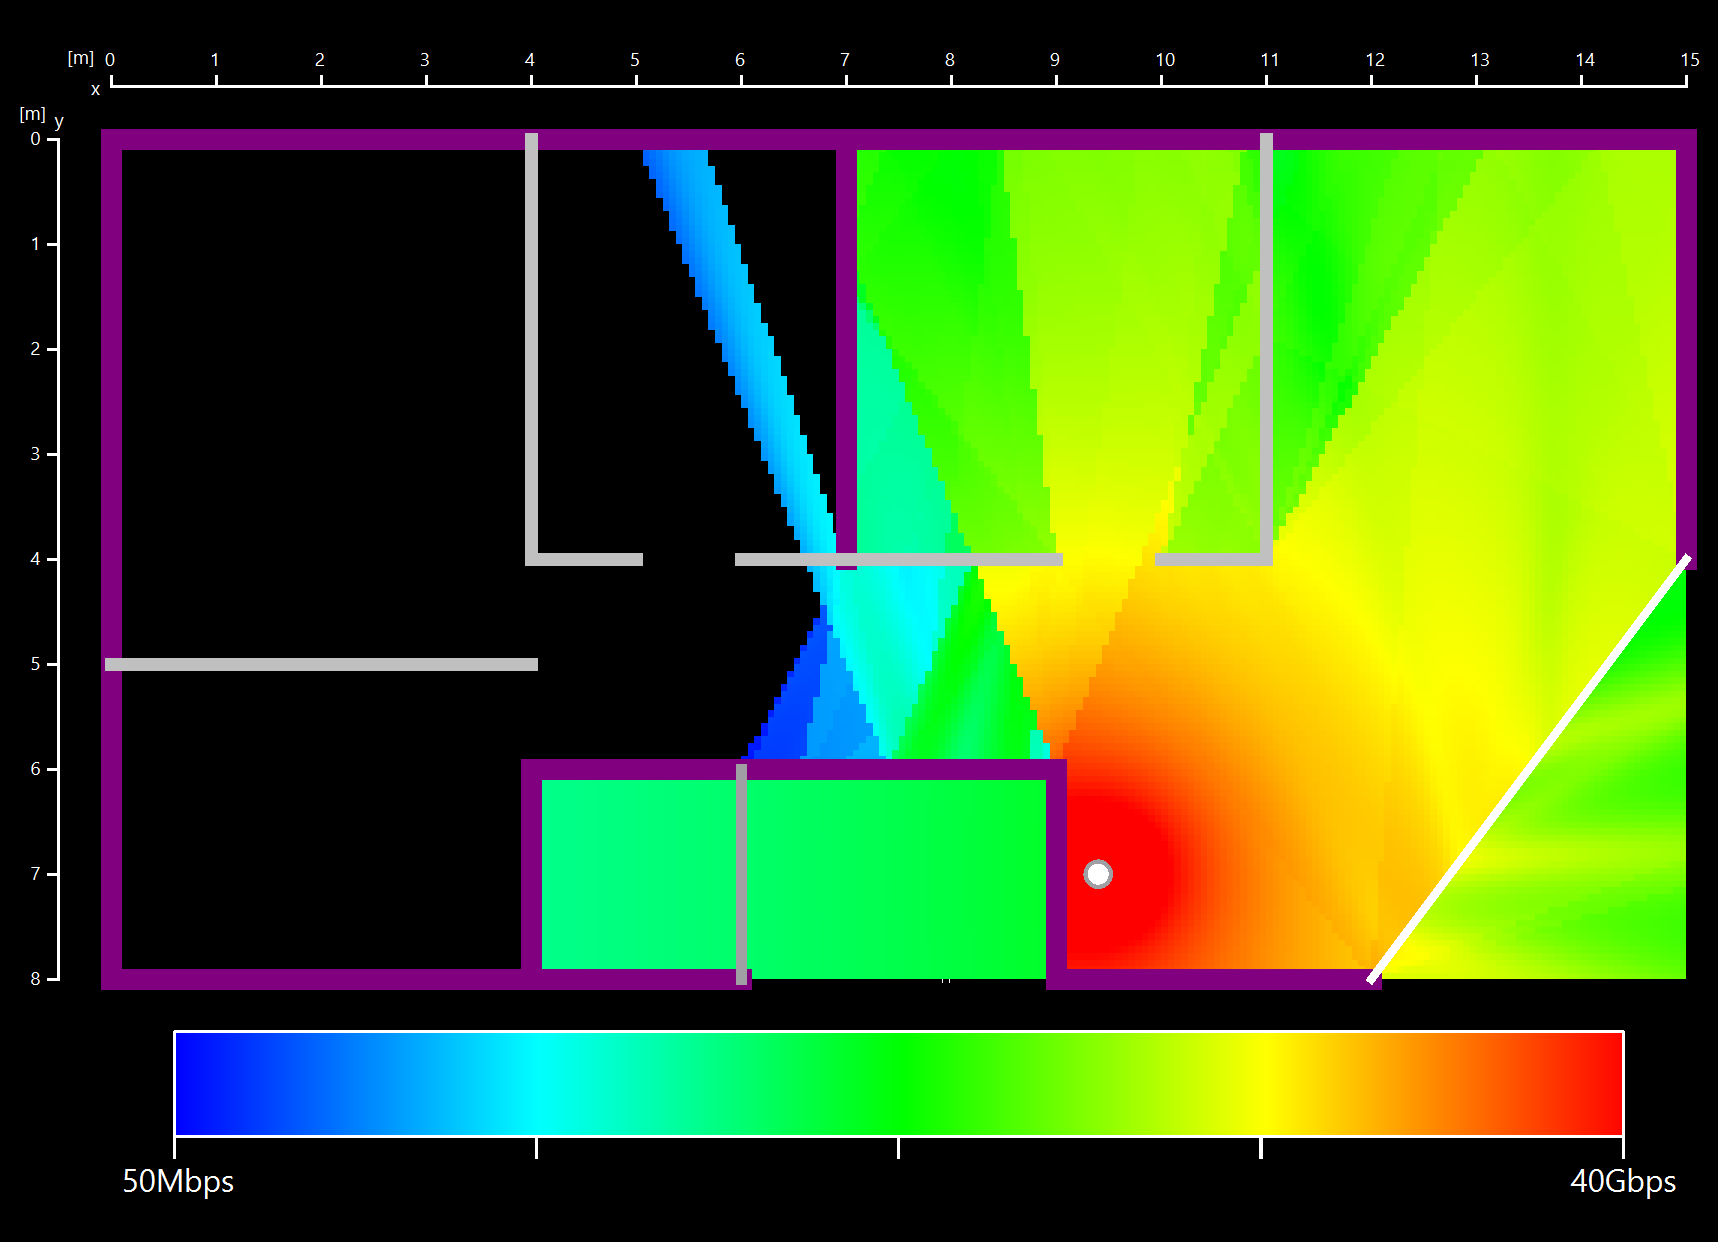
\includegraphics[width=0.68\textwidth]{latex/images/highres-without-lift.png}
    \caption{Couverture débit binaire station de base salon, sans ascenseur}
    \label{fig:simu-emplacement-defaut-sansasc}
\end{figure}

\subsubsection{Avec ascenseur}

\begin{figure}[H]
    \centering
    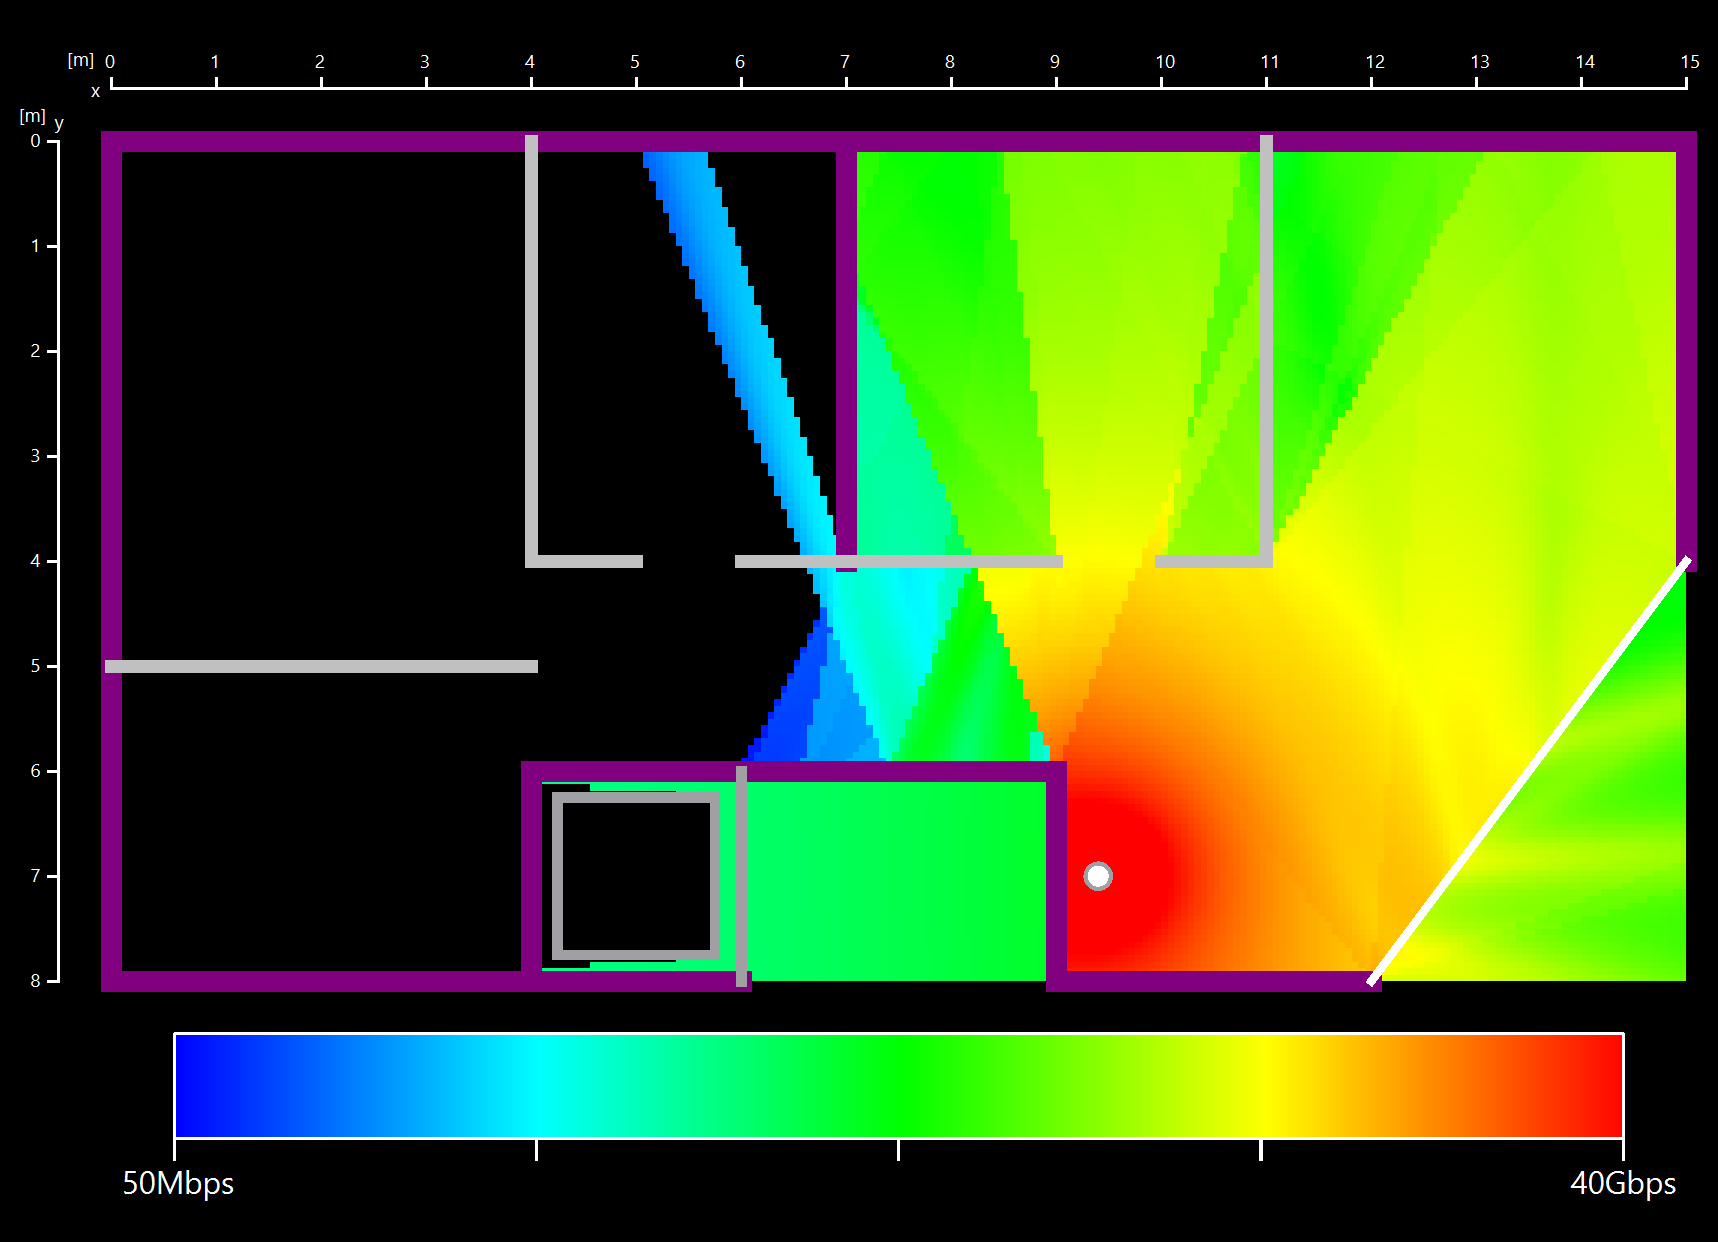
\includegraphics[width=0.6\textwidth]{latex/images/highres-with-lift.png}
    \caption{Couverture débit binaire station de base salon, avec ascenseur}
    \label{fig:simu-emplacement-defaut-avecasc}
\end{figure}

\begin{figure}[H]
    \centering
    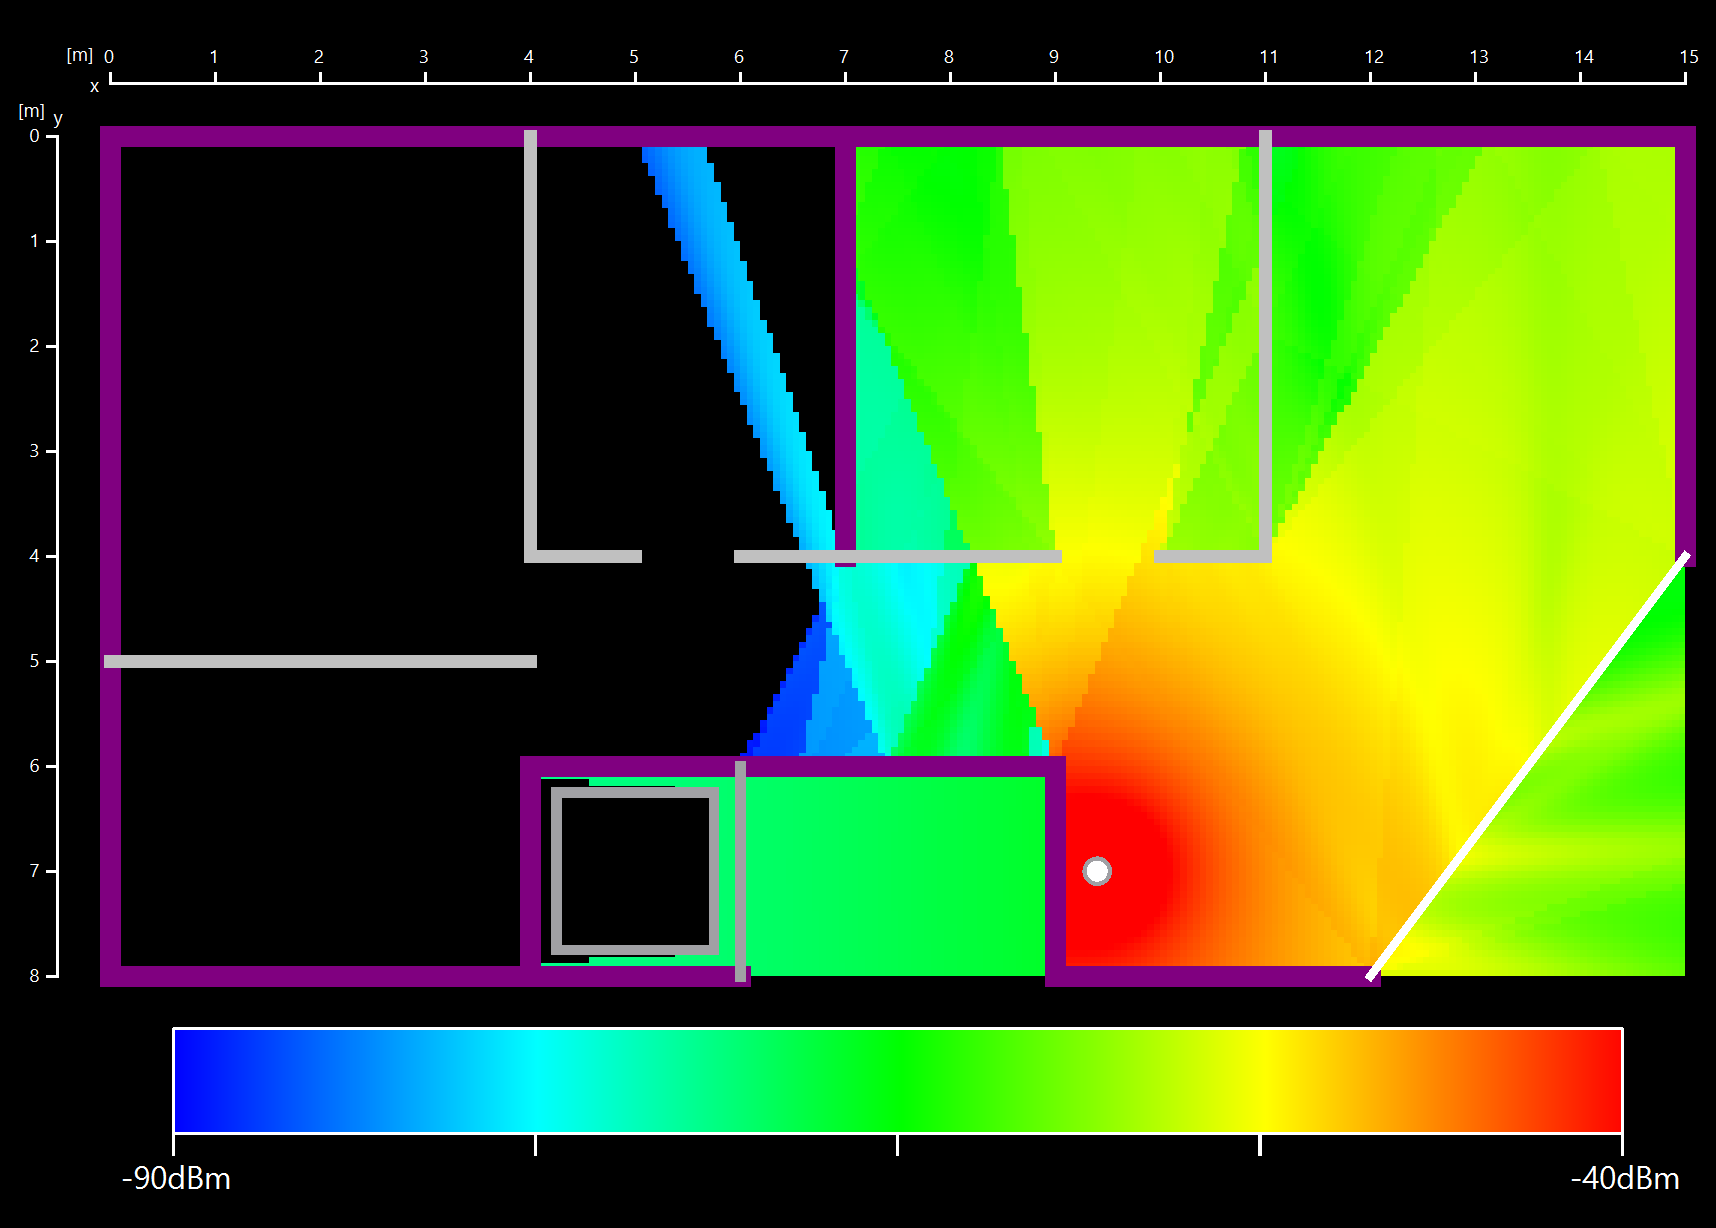
\includegraphics[width=0.6\textwidth]{latex/images/highres-with-lift-power.png}
    \caption{Couverture puissance station de base salon, avec ascenseur}
    \label{fig:simu-emplacement-defaut-avecasc-puissance}
\end{figure}

On observe qu'il n'y a pas de différence visuelle entre la couverture puissance et la couverture débit binaire
car l'échelle est définie comme le logarithme du débit binaire, ou la puissance en dBm, donc l'amplitude de couleur est la même.
%(en log) car ces deux grandeurs sont proportionnelles:\\
%$$\mathrm{bitrate}_{dB} = \mathrm{minBitrate}_{dB} + \frac{\mathrm{power}_{dBm}-\mathrm{minPower}_{dBm}}{\mathrm{maxPower}_{dBm}-\mathrm{minPower}_{dBm}} (\mathrm{maxBitrate}_{dB}-\mathrm{minBitrate}_{dB})$$


%\mintinline{cpp}{btrt_dB = min_btrt_dB + ((pwr_dBm - min_pwr_dBm) / (max_pwr_dBm - min_pwr_dBm)) * (max_btrt_dB - min_btrt_dB)}
% -----------


% ---- chambre 1 ----
%\subsection{Emplacement chambre 1}
%La station de base se trouve en (0,5 ; 4)m.
%
%\subsubsection{Sans ascenseur}
%
%\begin{figure}[H]
%    \centering
%    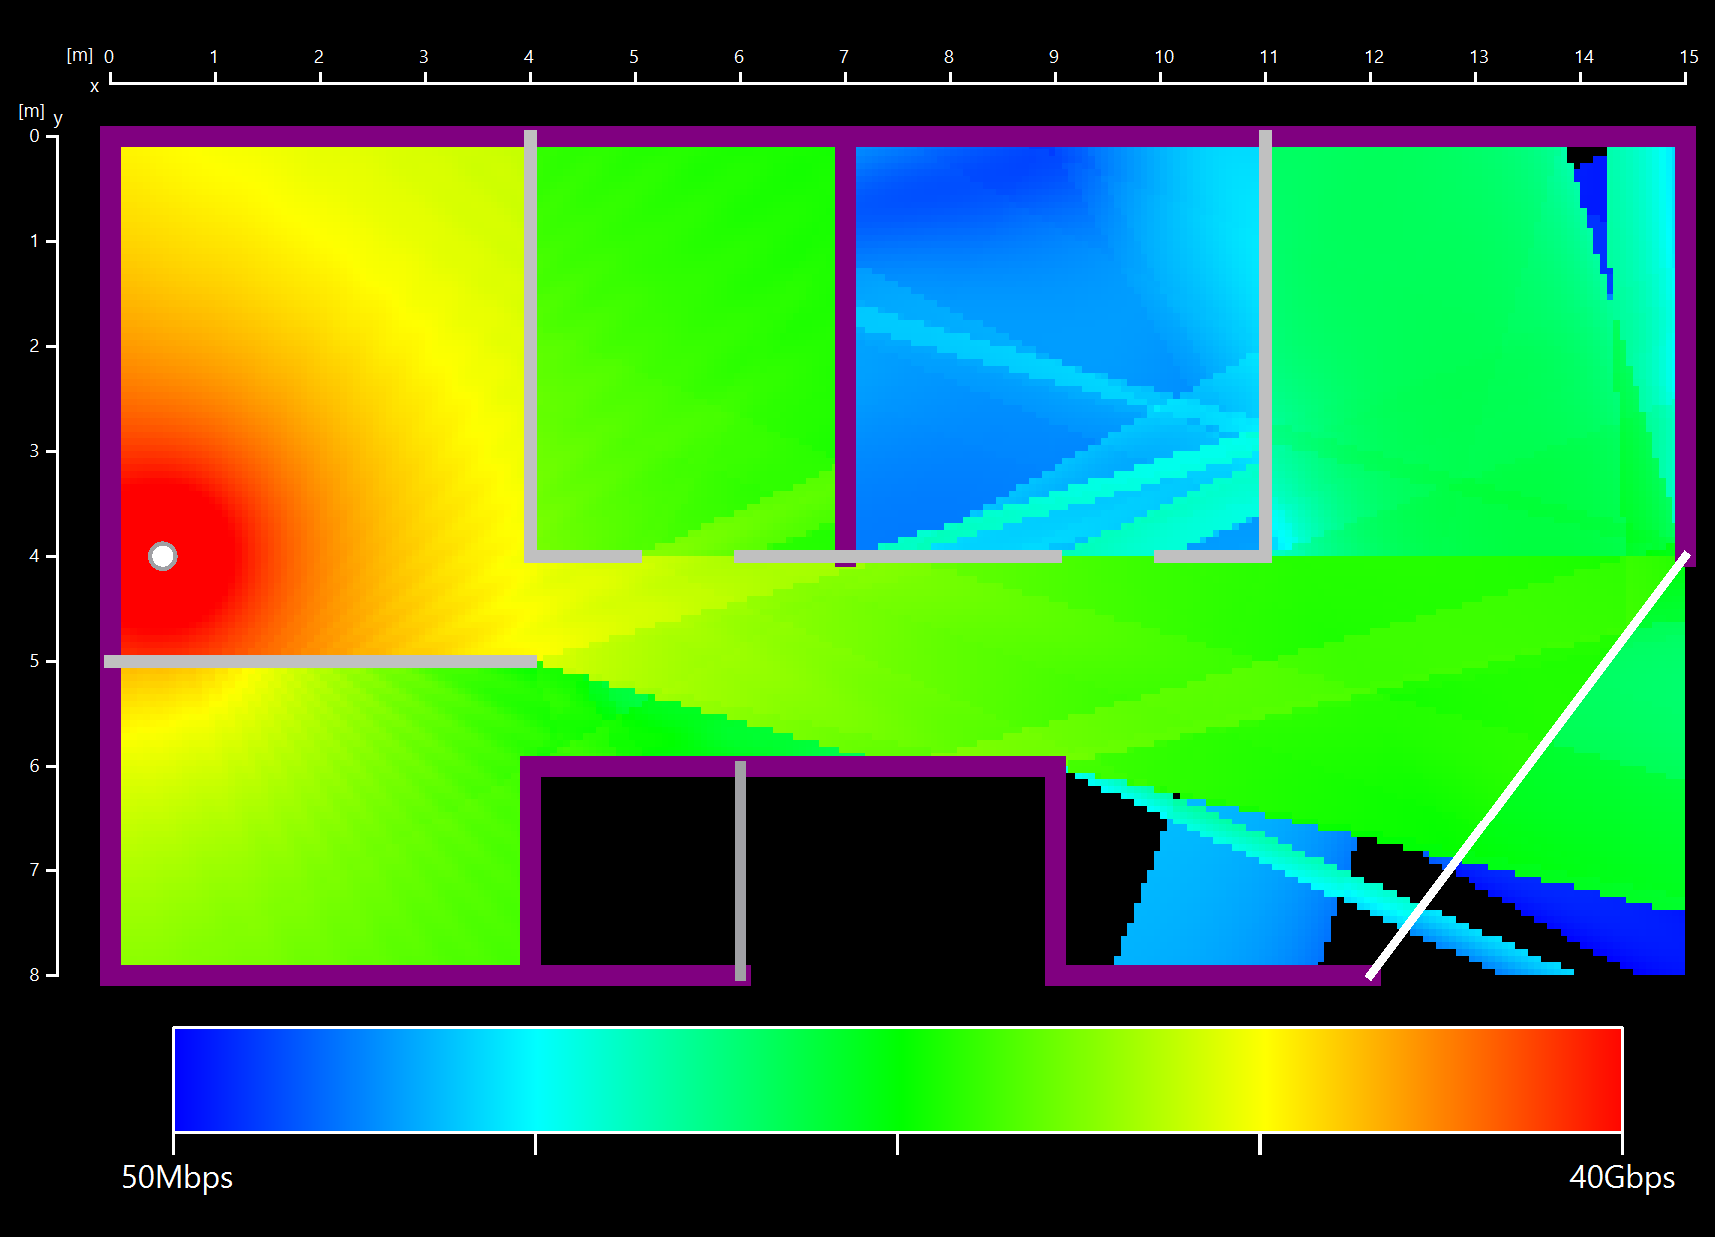
\includegraphics[width=0.6\textwidth]{latex/images/highres-chambre1-without-lift.png}
%    \caption{Couverture station de base chambre 1, sans ascenseur}
%    \label{fig:simu-emplacement-chambre1-sansasc}
%\end{figure}
%\subsubsection{Avec ascenseur}
%
%\begin{figure}[H]
%    \centering
%    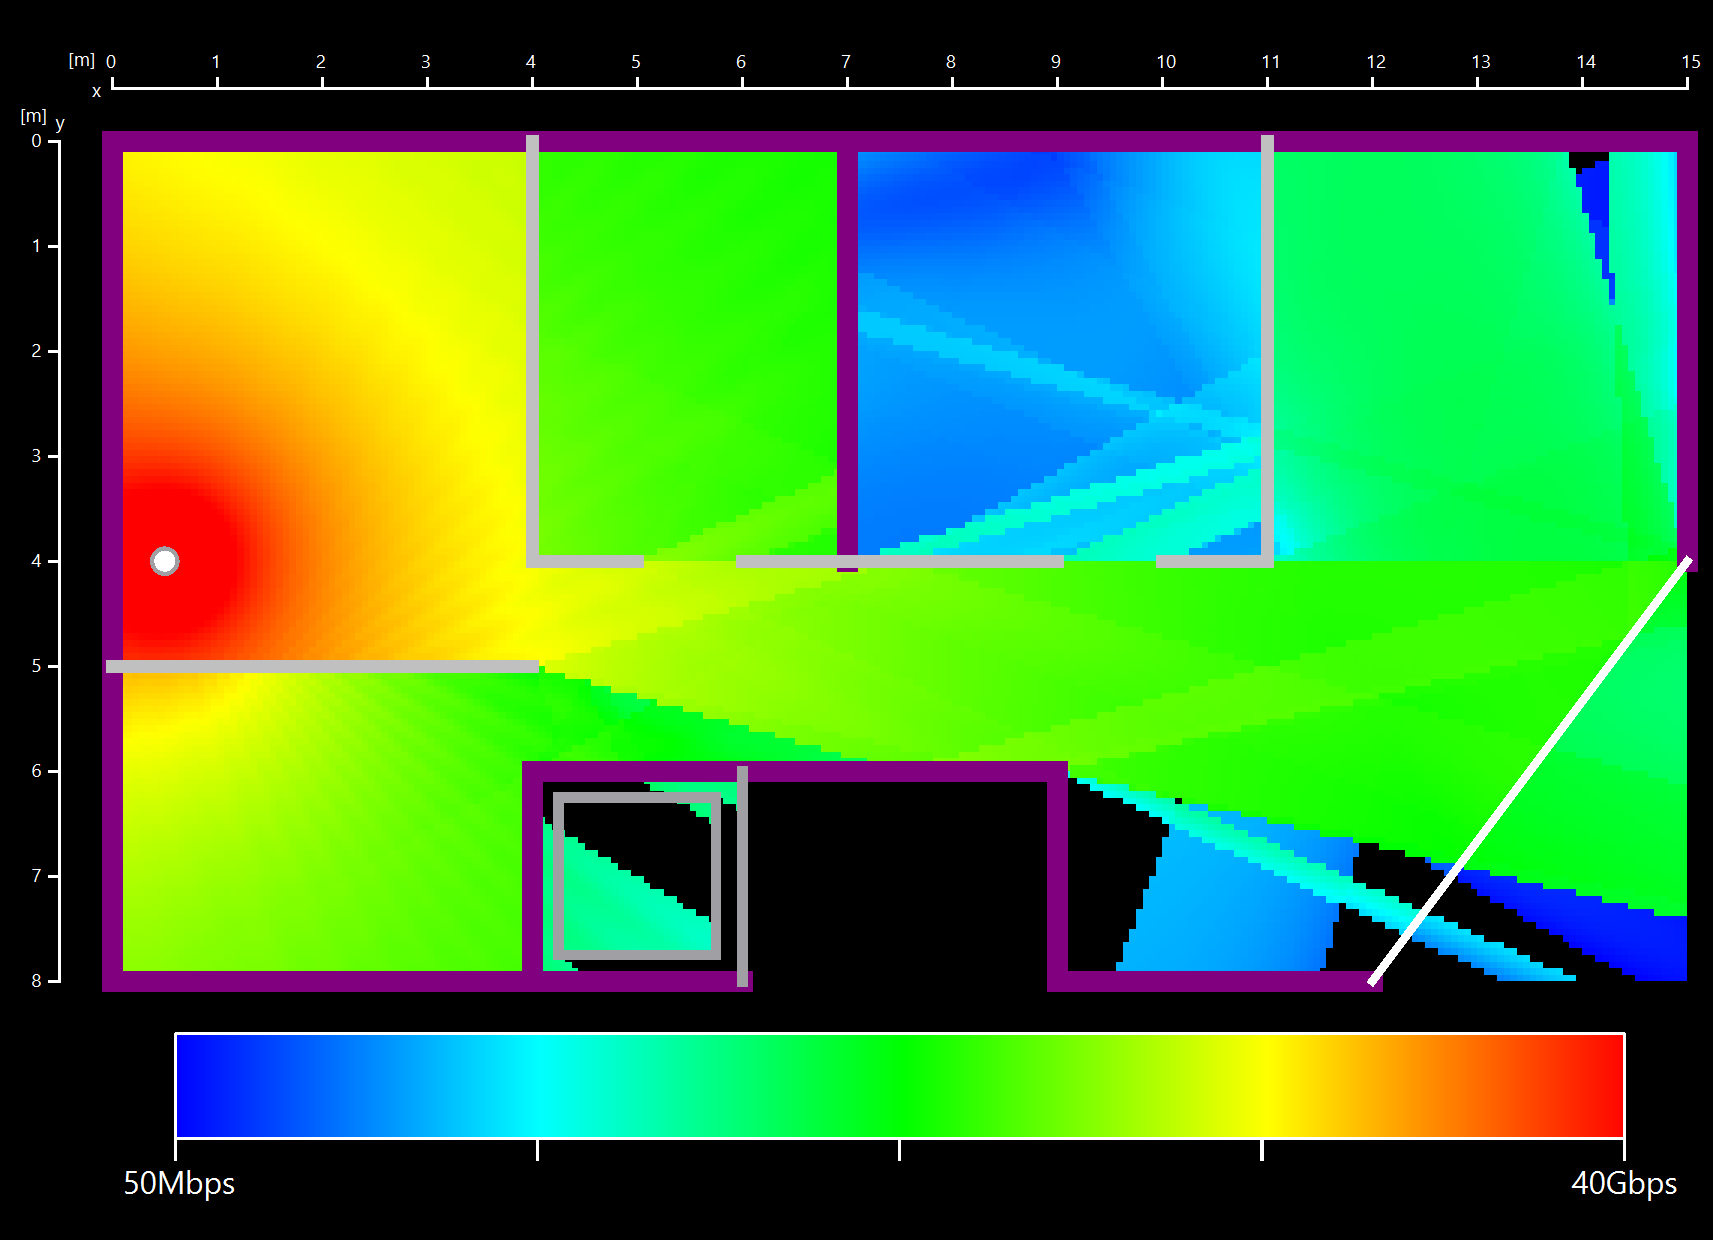
\includegraphics[width=0.6\textwidth]{latex/images/highres-chambre1-with-lift.png}
%    \caption{Couverture station de base chambre 1, avec ascenseur}
%    \label{fig:simu-emplacement-chambre1-avecasc}
%\end{figure}
% -----------------


\section{Suggestions placement station de base}

Afin de trouver un emplacement optimal pour la station de base, il est intéressant de réaliser un algorithme trouvant cette position. Nous profitons de la vitesse d'exécution de notre simulation en déterminant l'emplacement ayant la plus haute moyenne des puissances des cellules via une méthode d'optimisation en \textit{brute-forcing}, c'est-à-dire nous itérons à travers toutes nos positions de station de base, et gardons seulement la meilleure. Notre algorithme d'optimisation nous indique qu'un emplacement optimal est (6.5, 4.5)m, la résolution basse a été utilisée, soit des cellules de $0,5\mathrm{m}\times0,5\mathrm{m}$.

Cet emplacement optimal \textbf{théorique} au milieu de l'appartement offre une large couverture, dû à son placement central et à sa plus grande distance à tous les murs en béton.

% ---- couloir ----
%\subsection{Emplacement couloir}
%La station de base se trouve en (7 ; 5)m.
%\subsubsection{Sans ascenseur}
\begin{figure}[H]
    \centering
    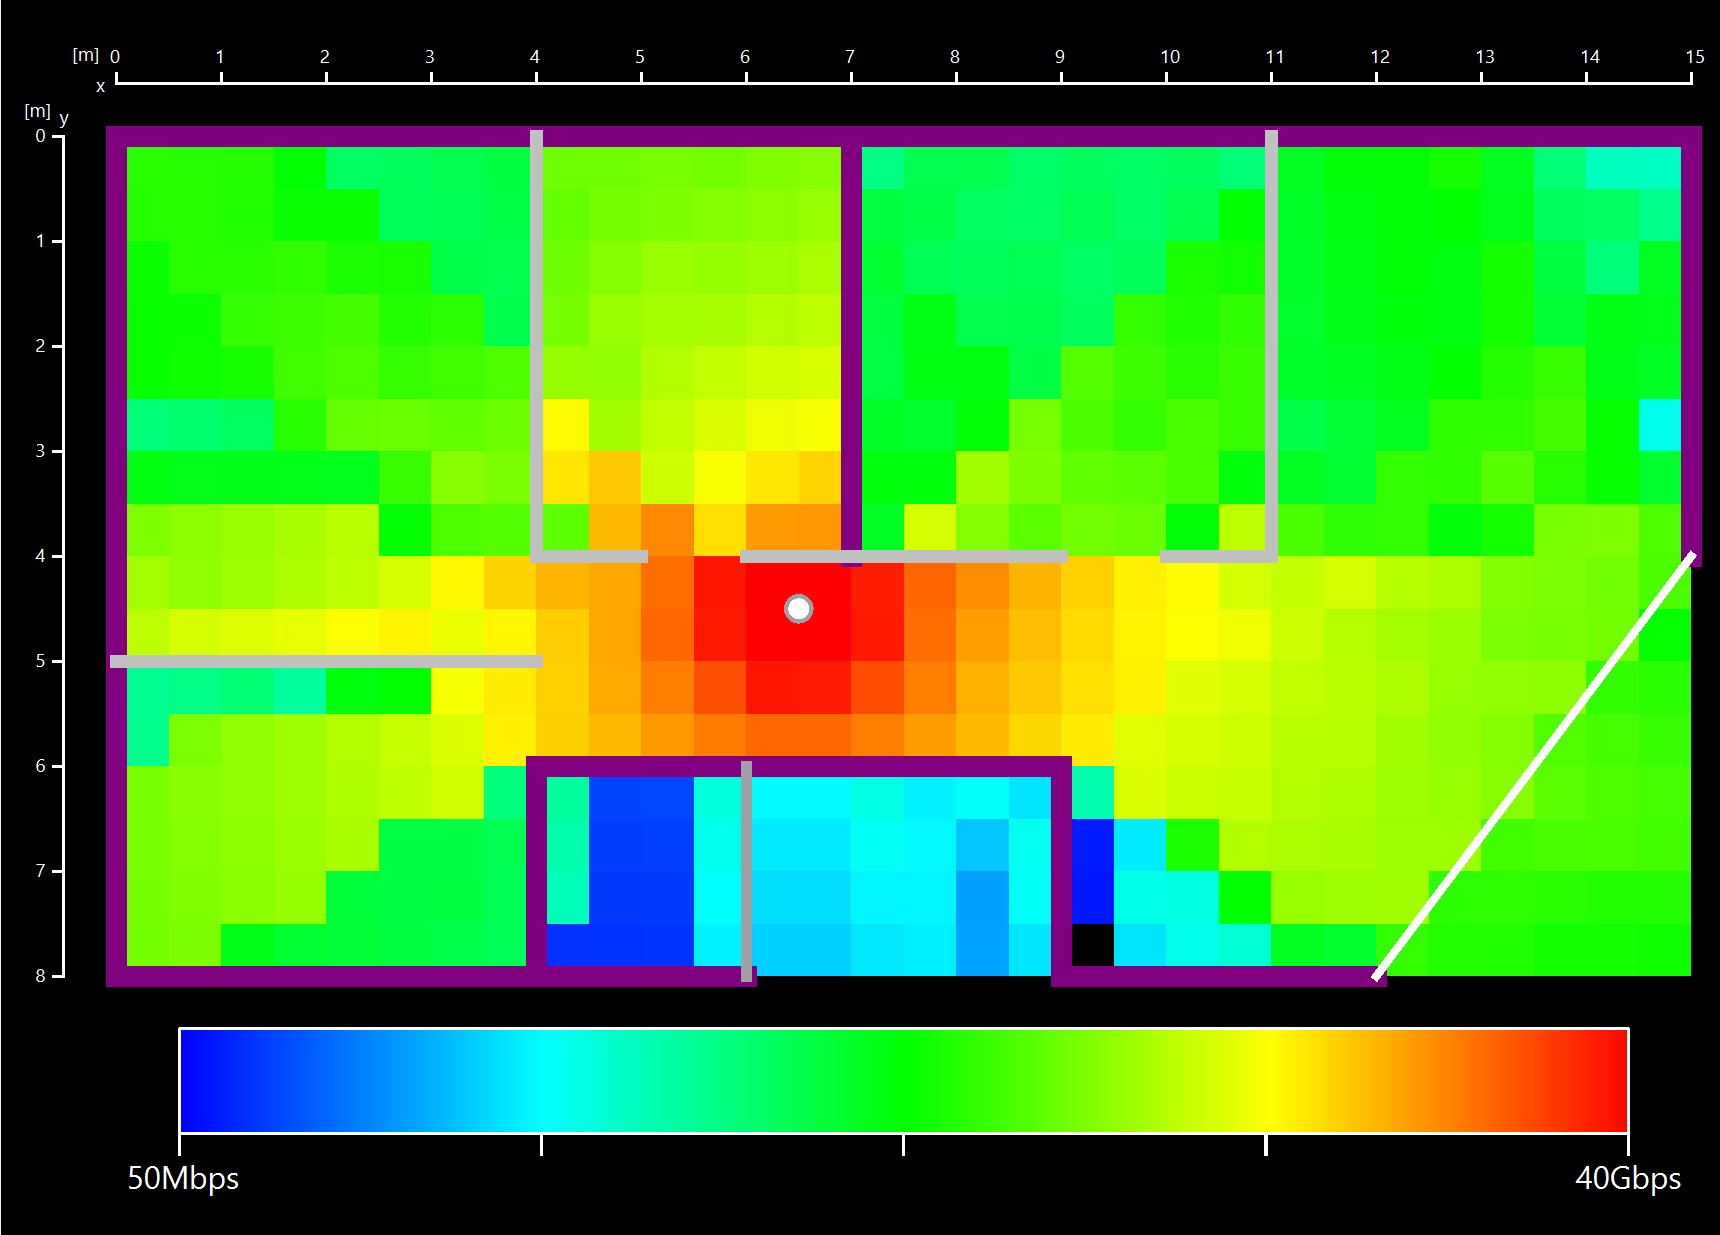
\includegraphics[width=0.6\textwidth]{latex/images/opti-without-lift.png}
    \caption{Couverture débit binaire station de base optimale, sans ascenseur}
    \label{fig:simu-emplacement-couloir-sansasc}
\end{figure}
%\subsubsection{Avec ascenseur}
\begin{figure}[H]
    \centering
    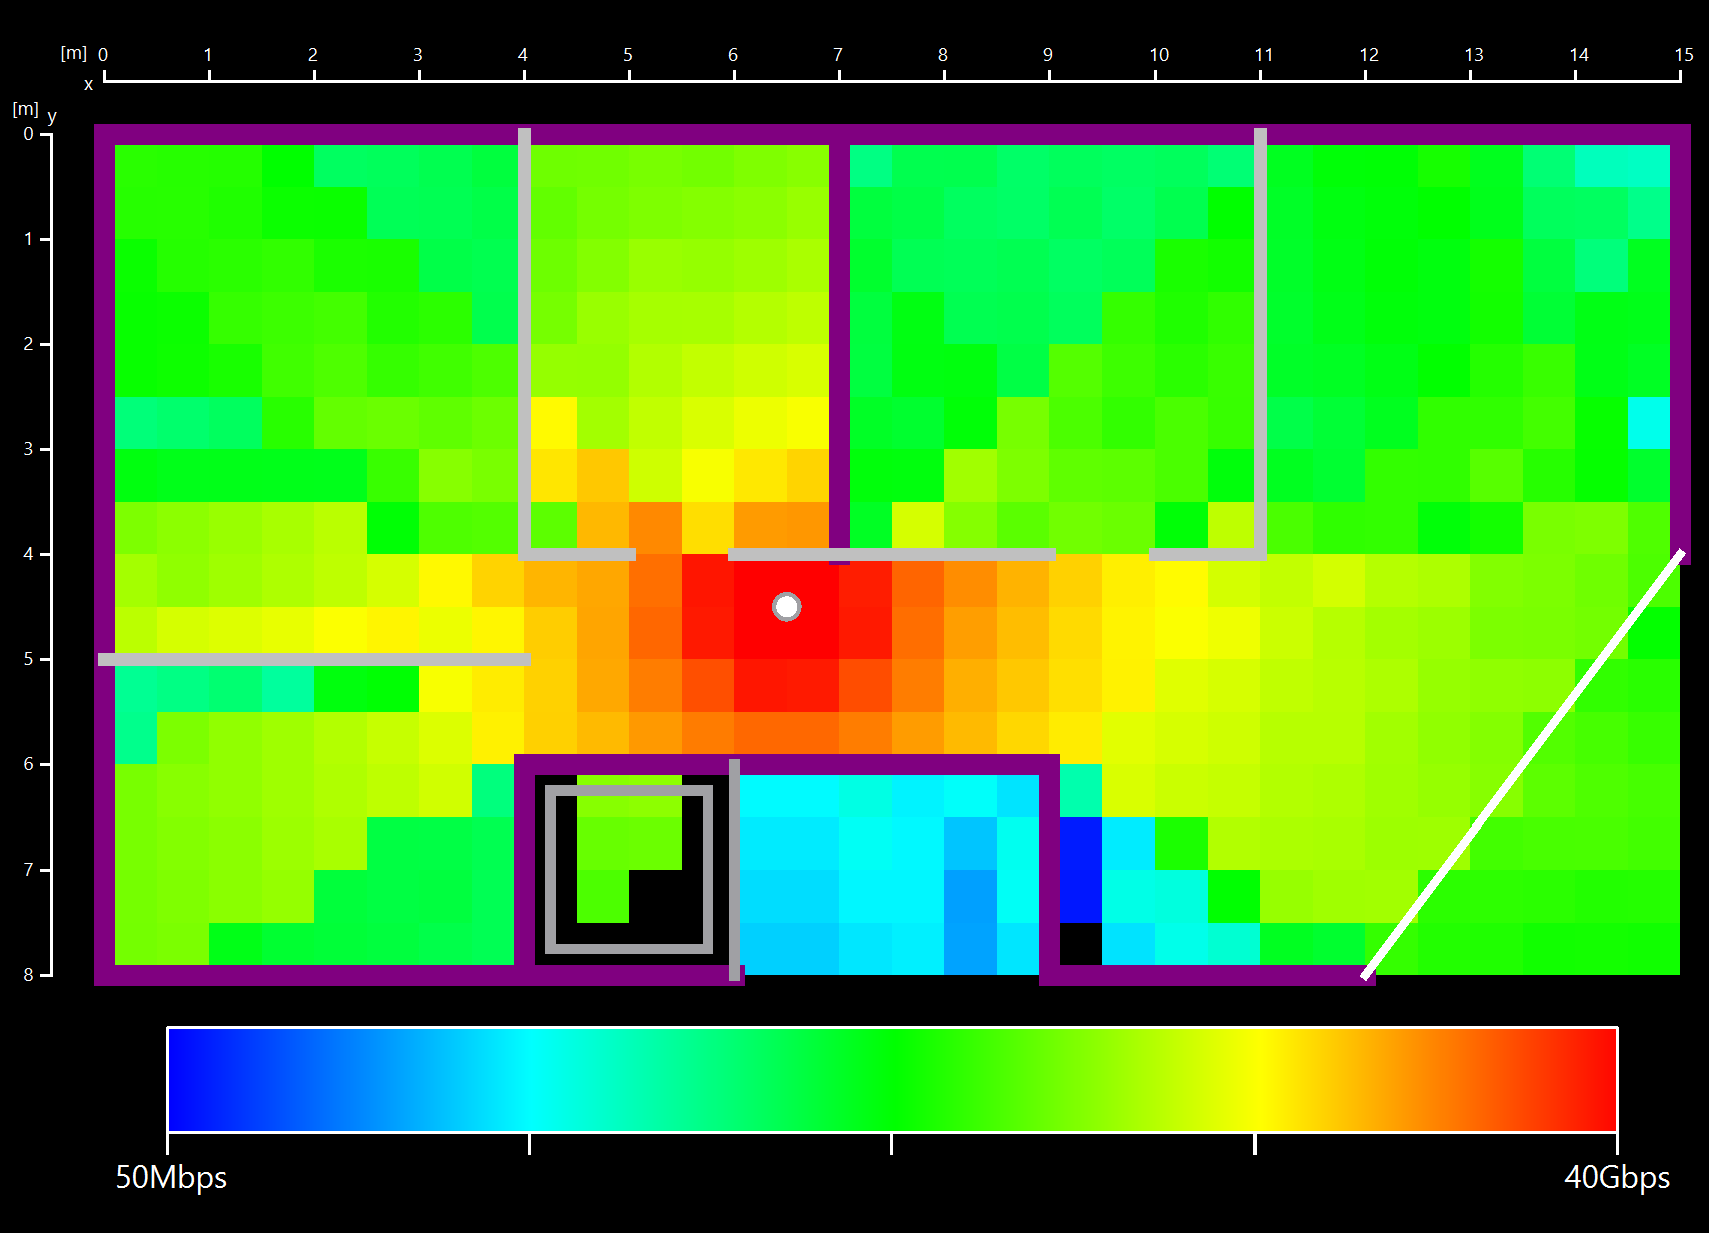
\includegraphics[width=0.6\textwidth]{latex/images/opti-with-lift.png}
    \caption{Couverture débit binaire station de base optimale, avec ascenseur}
    \label{fig:simu-emplacement-couloir-avecasc}
\end{figure}
% -----------

Un emplacement au milieu d'une pièce est évidemment non favorable en pratique, car loin de prises de courant et réseau, et nécessite aussi sans doute de placer la station de base au plafond ce qui engendre un travail supplémentaire lors de l'installation et un aspect esthétique moindre. Nous privilégions alors un emplacement proche d'un mur, sans doute sur un meuble, par soucis pratique.


L'emplacement proche de celui du projet par défaut par exemple à (9.4, 6.4)m semble être un emplacement réaliste et efficace et donc meilleur à utiliser en \textbf{pratique}. La station de base se trouve dans le salon de l'appartement, un lieu où est souvent situé le raccordement internet, et là où sont majoritairement utilisés les appareils sans-fil lors de besoins élevés en débit binaire (téléchargements, vidéos, etc). De plus, la cuisine et la salle à manger sont bien couvertes (deux autres pièces qui sont plus enclines à une utilisation du réseau Wi-Fi par les habitants, contrairement aux chambres et salle de bain). Voir Figures [\ref{fig:simu-emplacement-defaut-sansasc}] et [\ref{fig:simu-emplacement-defaut-avecasc}] pour sa couverture de débit binaire.\\


\section{Suggestion nombre de stations de base}
...
Nous pouvons ré...
% système mesh

\begin{figure}[H]
    \centering
    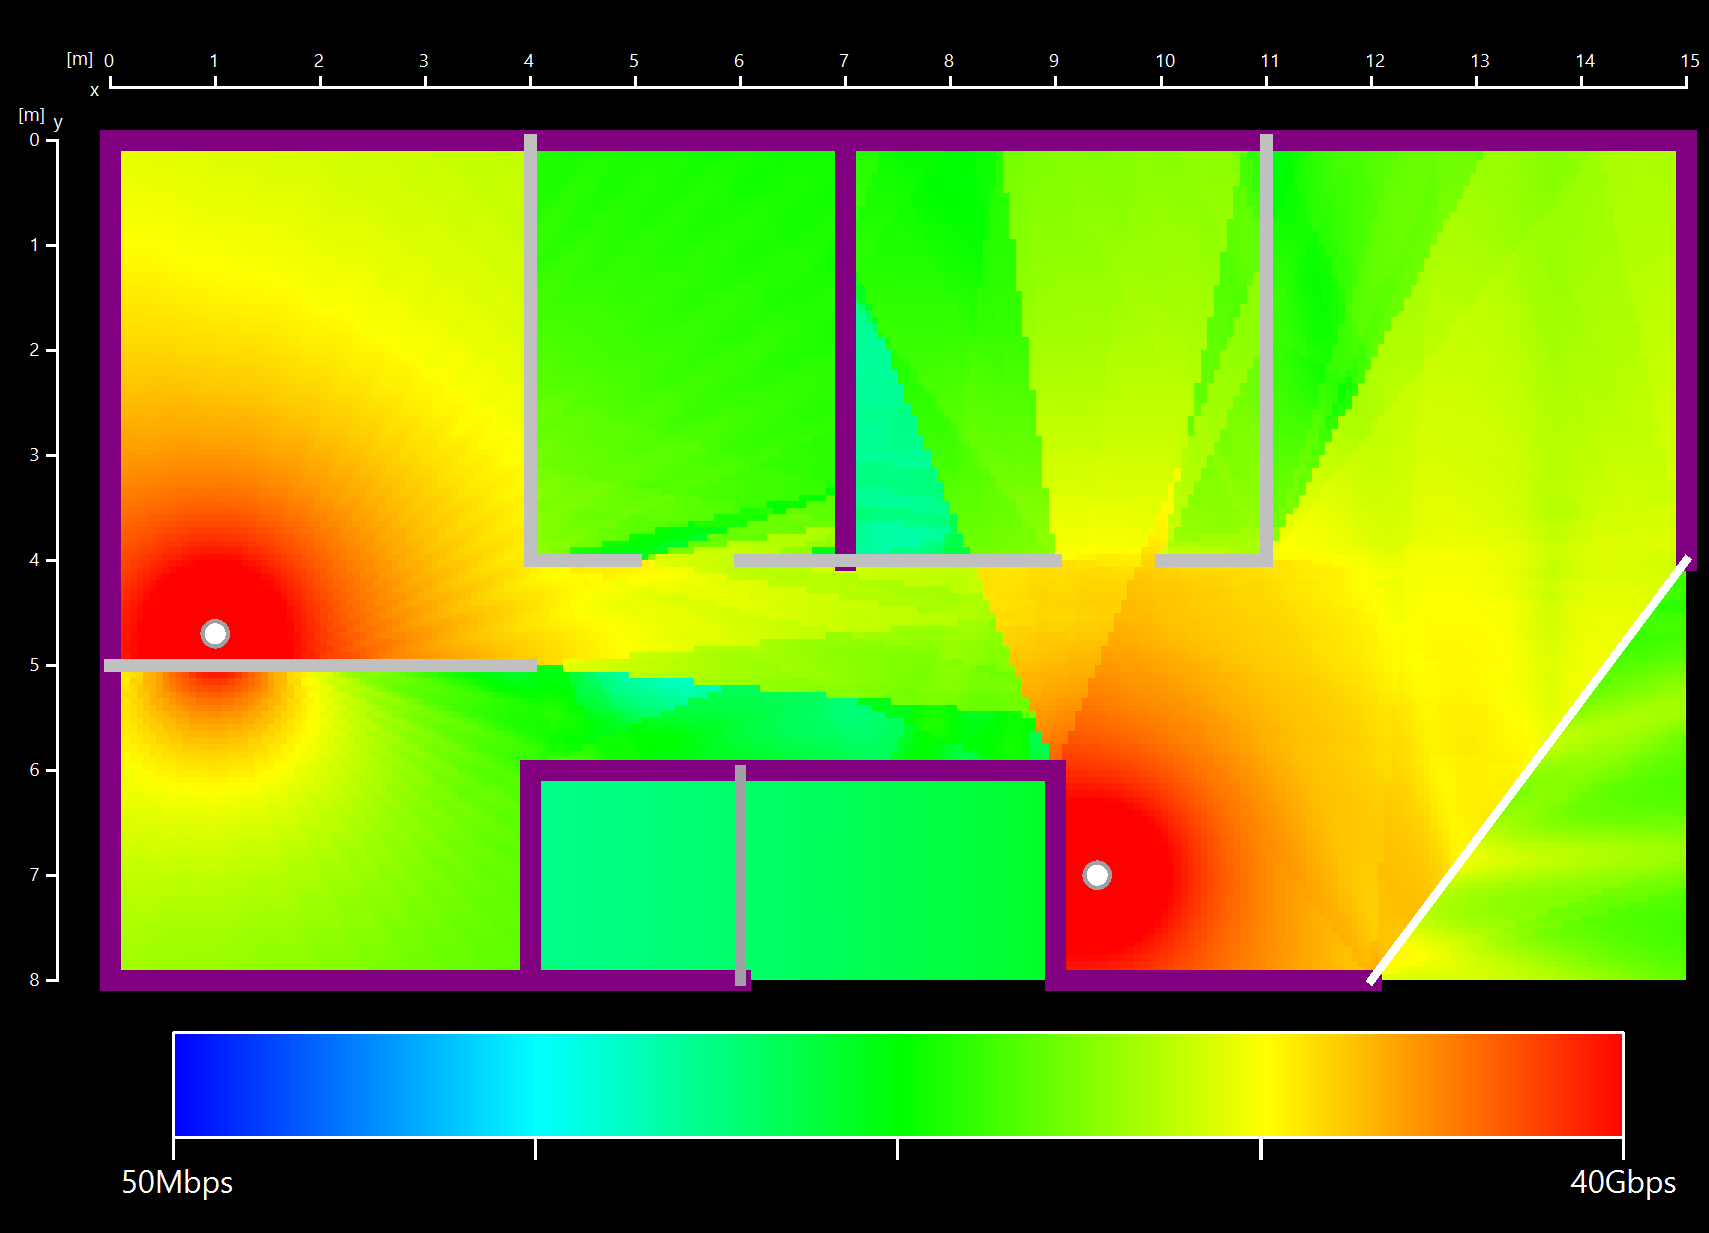
\includegraphics[width=0.6\textwidth]{latex/images/multiple-tx-highres-without-lift.png}
    \caption{Exemple de couverture débit binaire pour deux stations de base, sans ascenseur}
    \label{fig:simu-two-tx-without-lift}
\end{figure}

Cependant, comme notre modèle ne prend pas en compte d'éventuelles interférences entre les différentes stations de base, il est donc \textbf{théoriquement} avantageux d'avoir le plus de station de base possible, ce qui n'est pas réaliste.

\section{Critique de la simulation}
% TODO ?
% parler du fait que les murs sont rarement direct en béton (en général du placo par dessus), présence de meubles, absence de la diffraction, pas de beam-forming, etc...

Tout d'abord, on peut observer qu'un débit binaire non-nul est présent à côté de l'ascenseur, ainsi que dans sa cage ou dans lui-même. Ce résultat ne devrait pas se produire dû à la présence d'épais murs en béton ainsi que de la ou des parois métalliques constituant l'ascenseur. Cette erreur a malheureusement une origine inconnue, il se peut qu'elle survienne à cause d'un \textbf{bug} des coins des murs, où des ondes passeraient. Bien des essais et des réecritures ont été tentées, mais sans succès. Essayer de résoudre ce problème fut une des choses qui prit le plus de temps durant la réalisation du projet, plus de détails sur les différents essais de résolution sont présents dans l'\textbf{Annexe [\ref{discussion-debit-critique}]}.

Ensuite, cette simulation repose sur de nombreuses simplifications et approximations. En effet, l'appartement ne présente pas d'obstacle de type meubles, ne possède aucune autre fenêtre (en plus de la baie vitrée oblique), des murs en béton sont normalement recouverts d'une couche de plâtre (affectant alors la réflexion différemment du béton). 

De plus, la simulation considère une antenne parfaitement omnidirectionnelle dans le plan étudié. 

Enfin, la simulation ne prend pas en compte la diffraction, et ignore les technologies maintenant très répandues dans les antennes Wi-Fi tel que le \textit{beam-forming} ou encore le \textit{MIMO}.
